\chapter{Návrh metody detekce karbohydrátů}

Příjem karbohydrátů způsobuje zvýšení hladiny koncentrace glukózy v krvi, které je nutné kompenzovat podáním inzulinu. Včasnou detekcí může systém upravit množství podávaného inzulinu tak, aby nedošlo k hyperglykémii.

Detekce karbohydrátů je na základě dat intersticiální glukózy měřené senzorem CGMS a její derivace. Pro detekci jsem zvolil tyto 3 metody:
\begin{itemize}
\setlength\itemsep{0em}
\item Long short-term memory neuronová síť (kapitola \ref{ch:lstm})
\item Lineární a kvadratická diskriminační analýza (kapitola \ref{ch:lda_qda})
\item Detekce hran pomocí thresholdů 1. diference hodnot intersticiální glukózy \\(kapitola \ref{ch:threshold})
\end{itemize}

\section{Rekurentní neuronové sítě}
\label{ch:lstm}

Rekurentní neuronové sítě jsou vhodné pro predikci sekvenčních dat (například časové řady). Vyznačují se tím, že si předávají informaci o předchozím stavu (aktivaci skryté vrstvy):

$H_{t}=\sigma (W_{h}H_{t-1}+W_{x}X_{t}+b)$

\noindent kde $W$ jsou váhy a $b$ je bias. Neurony, které takto uchovávají svůj stav, se nazývají buňky. 

\begin{figure}[H]
\caption{Rekurentní neuronová síť}
\label{fig:rnn}
\centering
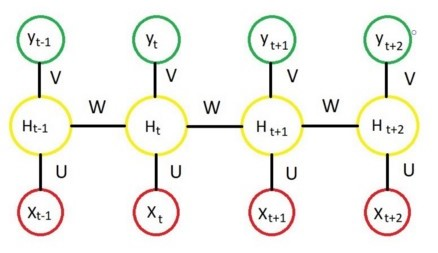
\includegraphics[width=0.65\textwidth]{img/cho/rnn.jpeg}\\
\textit{Zdroj: https://medium.com/}
\end{figure}

Riziko RNN spočívá v náchylnosti vzniku jevu označovaného jako mizející nebo explodující gradient vznikajícího při zpětné propagaci, kdy hodnoty exponenciálně klesají nebo rostou. To je z důvodu, že se chyba propaguje přes všechny iterace. Tento problém eliminuje long short-term memory nebo gated recurrent unit neuronová síť.

\subsection{Long short-term memory}

Long short-term memory neuronová síť (LSTM) je speciální případ rekurentní neuronové sítě. V každé iteraci si buňka uchovává dodatečnou informaci nazvanou \textit{memory}. 

Nejprve se ze vstupního vektoru $X_{t}$ a stavu předchozí buňky $H_{t-1}$ spočte Forget gate $f_{t}$, Candidate layer $\bar{C}_{t}$ Input gate $I_{t}$ a Output gate $O_{t}$ \citep{cho.lstm}:

$f_{t}=\sigma(X_{t} \otimes U_{f}+H_{t-1} \otimes W_{f})$\\\indent
$\bar{C}_{t}=tanh(X_{t} \otimes U_{c}+H_{t-1} \otimes W_{c})$\\\indent
$I_{t}=\sigma(X_{t} \otimes U_{i}+H_{t-1} \otimes W_{i})$\\\indent
$O_{t}=\sigma(X_{t} \otimes U_{u}+H_{t-1} \otimes W_{u})$

\noindent kde $W$ a $U$ jsou váhové vektory. Následně se spočte \textit{memory} prvek $C_{t}$:

$C_{t}=f_{t} \otimes C_{t-1} \oplus I_{t} \otimes \bar{C}_{t}$

\noindent a výstupní stav $H_{t}$:

$H_{t}=O_{t} \otimes tanh(C_{t})$

Diagram LSTM buňky je na obrázku \ref{fig:lstm_cell}.

\begin{figure}[H]
\caption{LSTM buňka}
\label{fig:lstm_cell}
\centering
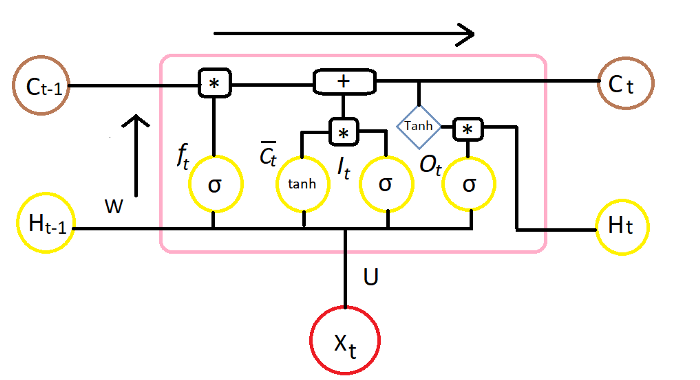
\includegraphics[width=0.9\textwidth]{img/cho/lstm_cell.png}
\textit{Zdroj: https://medium.com/}
\end{figure}

\subsection{Gated recurrent unit}

Gated recurrent unit neuronová síť (GRU) využívá Update gate $z_{t}$ a Reset gate $r_{t}$. Ty určují která informace bude propagována na výstup. Mohou tak vytěžit relevantní informace. Update a reset gate se spočte \citep{cho.gru}:

$z_{t}=\sigma(W_{z}x_{t} + U_{z}h_{t-1})$\\\indent
$r_{t}=\sigma(W_{r}x_{t} + U_{r}h_{t-1})$

\noindent kde $W$ a $U$ jsou váhové vektory. Následně se spočte relevantí informace z předchozího stavu $\bar{h}_{t}$:

$\bar{h}_{t}=tanh(W_{h}x_{t} + U_{h}(r_{t} \otimes h_{t-1}))$

\noindent a výstupní stav $h_{t}$:

$h_{t}=z_{t} \otimes h_{t-1} + (1-z_{t}) \otimes \bar{h}_{t}$

Diagram GRU buňky je na obrázku \ref{fig:gru_cell}.

\begin{figure}[H]
\caption{GRU buňka}
\label{fig:gru_cell}
\centering
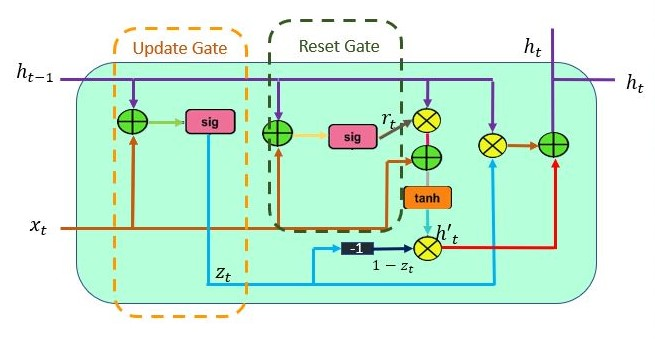
\includegraphics[width=1\textwidth]{img/cho/gru_cell.jpg}
\textit{Zdroj: https://www.pluralsight.com/}
\end{figure}

\subsection{Model}

Pro detekci karbohydrátů jsem sestavil sekvenční keras model\footnote{Keras je nadstavba nad knihovnou TensorFlow pro neuronové sítě} se čtyřmi vrstvami:
\begin{itemize}
\setlength\itemsep{0em}
\item Obousměrná LSTM nebo GRU
\item Dropout(0,5)
\item Dense(128)
\item Dense(1)
\end{itemize}

První vrstvou je rekurentní neuronová síť. Ta může být buď LSTM nebo GRU. Tato vrstva má 128 neuronů, dropout 0,2 a aktivační funkcí je hyperbolický tangens. Vstupem vrstvy je časové okno N vstupních prvků velikosti W. Tvar vstupních dat je WxN:

$\begin{bmatrix}
X^{1}_{1} & X^{2}_{1} & ... & X^{N}_{1}\\
X^{1}_{2} & X^{2}_{2} & ... & X^{N}_{2}\\
... & ... & ... & ...\\
X^{1}_{W} & X^{2}_{W} & ... & X^{N}_{W}
\end{bmatrix}$

Dropout vrstva s \textit{rate=0,2} náhodně nastaví některé vstupy na nulu v poměru 0,2. Nevynulované vstupy jsou škálovány 1/(1-rate), takže součet všech vstupů je nezměněn. To zabrání přetrénování neuronové sítě. Droupout vrstva je aplikována pouze při trénování sítě. První Dense vrstva (propojení neuronů formou každý s každým) má 128 neuronů, aktivační funkce je \textit{relu}. Druhá Dense vrstva s jedním neuronem je výstupní.


\section{Lineární a kvadratická diskriminační analýza}
\label{ch:lda_qda}

Pro diskriminační analýzu jsem se rozhodl vzhledem k vysoké úspěšnosti a malému zpoždění, které dosáhli \citet{analyzaCHO.LDA} v článku \textbf{Pattern Recognition Reveals Characteristic Postprandial Glucose Changes: Non-Individualized Meal Detection in Diabetes Mellitus Type 1} (kapitola \ref{ch:analyzaCHO:lda}).

Diskriminační analýza slouží k rozdělení prvků do konečného počtu tříd na základě lineární kombinace charakteristických prvků. Pro klasifikaci potřebujeme znát posteriory tříd \textbf{P(Y|X)}. Pravděpodobnostní model \textbf{P(X|y=k)} pro každou třídu \textbf{k} lineární a kvadratické diskriminační analýzy je dán vícerozměrnou Gaussovo distribucí \citep{cho.book.lda}:

\scalebox{1.2}{$P(X|y=k)=\frac{1}{(2\pi)^{p/2}|\sum_{k}|^{\frac{1}{2}}}e^{-\frac{1}{2}(x-\mu_{k})^{T}\sum^{-1}_{k}(x-\mu _{k})}$}\\\\
kde \textbf{p} je počet prvků. Pro predikci je pak použito Bayesovo rozhodovací pravidlo \citep{cho.book.lda}:

\scalebox{1.2}{$P(y=k|x)=\frac{P(x|y=k)P(y=k)}{P(x)}=\frac{P(x|y=k)P(y=k)}{\sum_{l}{P(x|y=l)P(y=l)}}$}\\\\
kdy hledáme třídu s maximálním posteriorem.

Logaritmus posterioru pro kvadratickou diskriminační analýzu (QDA) je \citep{cho.book.lda}:

$P(y=k|x)=-\frac{1}{2}log|\sum_{k}|-\frac{1}{2}(x-\mu_{k})^{T}\sum^{-1}_{k}(x-\mu_{k})+logP(y=k)$\\\\
Predikovaná třída je ta, která má maximální logaritmický posterior.

Lineární diskriminační analýza (LDA) je speciální případ QDA, kdy předpokládáme, že třídy mají stejnou kovarianční matici. Logaritmus posterioru je pak vyjádřen \citep{cho.scikit.lda}:

$P(y=k|x)=-\frac{1}{2}(x-\mu_{k})^{T}\sum^{-1}(x-\mu_{k})+logP(y=k)$\\

Vstupem diskriminační analýzy může být buď množina prvků pro daný časový okamžik nebo časové okno jednoho prvku. Predikované třídy jsou příjem/nepříjem karbohydrátů. Ty dostaneme převedením sloupce karbohydrátů na booleanovskou proměnnou (0 je false, cokoli větší než 0 je true).

\subsection{Množina prvků}

Nejčastějším vstupem diskriminační analýzy je množina charakteristických prvků $X_{i}$. V tomto případě se diskriminační analýza snaží rozdělit prostor tak, aby odlišila jednotlivé třídy (viz obrázek \ref{fig:lda}).

\begin{figure}[H]
\caption{Rozdělení prostoru lineární diskriminační analýzou dvou prvků}
\label{fig:lda}
\centering
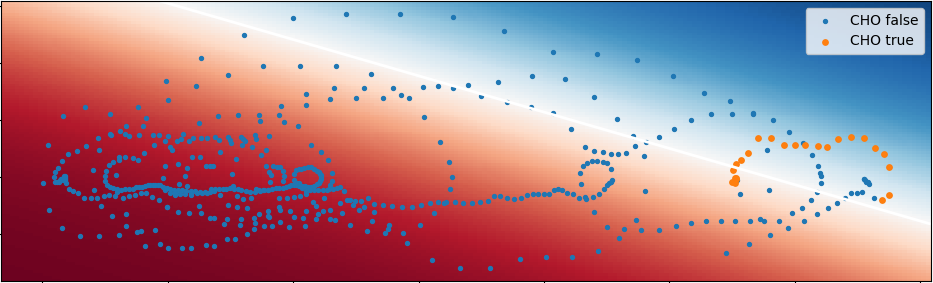
\includegraphics[width=1\textwidth]{img/cho/lda2.png}
\end{figure}

\subsection{Časové okno}

V případě časového okna muže být na vstupu pouze jediný prvek. To je dáno tím, že vstupem diskriminační analýzy je jedno-dimenzionální pole dat. Vstupní data mají tvar:

$\begin{bmatrix}
X_{i-W} & X_{i-W-1} & ... & X_{i-1} & X_{i}
\end{bmatrix}$

\noindent kde W je velikost časového okna. Časové okno jako vstupní data použili i \citet{analyzaCHO.LDA}.

Při experimentální implementaci diskriminační analýzy se mi nepodařilo dosáhnout stejných výsledků, jako autoři původního článku. Nejlepších výsledků dosahoval kvadratická diskriminační anaýza jejímž vstupem bylo dvou hodinové časové okno. Z testovacích 150 zadaných jídel jich detekovala 54 \% a falešně pozitivních detekcí bylo 155. Rozdílné výsledky mohou být dány tím, že původní metoda byla otestována pouze s daty predikovanými na základě Bergmanova modelu, ale ne s reálnými daty pacientů.

\section{Detekce hran průběhu intersticiální glukózy}
\label{ch:threshold}

Tato metoda detekuje vzestupné a klesající hrany průběhu intersticiální glukózy pomocí thresholdů první diference měřených hodnot intersticiální glukózy.

Derivace funkce $f'(x)$ v bodě $x$ je směrnicí tečny funkce $f(x)$ v daném bodě. Její hodnota je rovna tangens úhlu $\alpha$, který tečná svírá s osou x. Pakliže je funkce $f(x)$ v bodě $x$ rostoucí, $tg(\alpha)$ je kladný. Pokud je $f(x)$ klesající, $tg(\alpha)$ je záporný. Velikost derivace v bodě $x$ pak udává velikost změny $f(x)$, neboli říká, jak strmě funkce stoupá či klesá. Derivace funkce $f(x)$ v bodě $x_{1}$ můžeme vyjádřit jako:

\scalebox{1.2}{$f'(x) = \frac{d}{dx}f(x) = \lim_{x \to x_{0}} \frac{f(x)-f(x_{0})}{x-x_{0}}$}

Jelikož data ze senzoru CGMS jsou diskrétní, můžeme derivaci nahradit rovnicí první diference. Pro data intersticiální glukózy tak dostáváme vztah:

\scalebox{1.2}{$\Delta IST = \frac{IST_{t} - IST_{t-1}}{\Delta t}$}

Naměřená data intersticiální glukózy mohou být zatížena šumem a případně i dočasnými výchylkami hodnot glukózy. Každá taková výchylka pak má značný vliv na hodnotu derivace. Z toho důvodu je potřeba data před výpočtem vyhladit. Pro vyhlazení dat byl zvolen digitální Savitzky-Golay filtr. Každá podmnožina $2m+1$ prvků je vzorkována na polynom stupně $p (p\leq 2m)$ ve smyslu nejmenších čtverců \citep{cho.savgol}. Pro vyhlazení dat intersticiální glukózy jsem zvolil polynom stupně 3 a velikost podmnožiny 21. Vyhlazená data vidíme v grafu na obrázku \ref{fig:savgol}.

\begin{figure}[H]
\caption{Vyhlazená data intersticiální glukózy}
\label{fig:savgol}
\centering
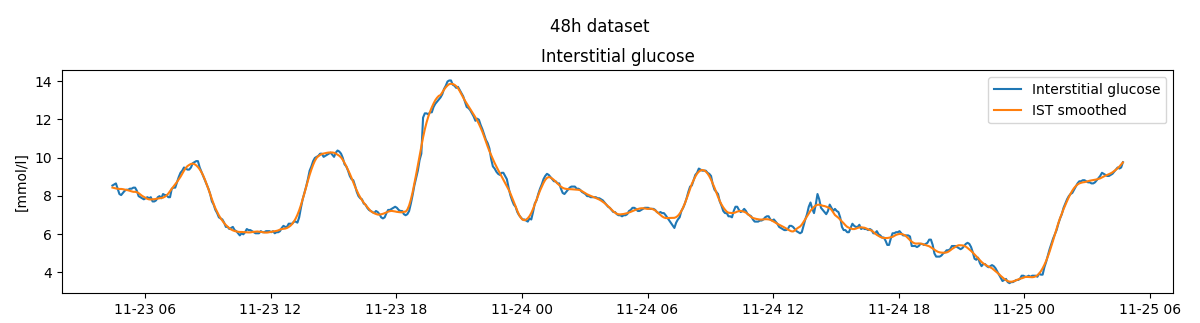
\includegraphics[width=1\textwidth]{img/cho/savgol.png}
\end{figure}

Následně se data ohodnotí. Pokud $\Delta IST$ překročí určitý threshold $th_{i}$, přiřadí se váha $w_{i}$. Takových dvojic thresholdů a vah může být libovolné množství. Experimentálně byla zjištěna kombinace thresholdů $th=[0.0125, 0.018]$ a vah $w=[2.25, 3]$.

Samotné ohodnocení podle thresholdů zachytí jakýkoli jednorázový větší výkyv v datech intersticiální glukózy. Jelikož příjem karbohydrátů se projevuje zvýšením glykémie v řádu desítek minut až hodin, chceme znát vývoj křivky intersticiální glukózy v čase. Z toho důvodu pro kladně ohodnocená data zvýšíme ohodnocení v případě, že předchozí hodnoty vykazují vzrůstající trend po dobu dvou hodin nazpět (tj. 24 hodnot, data jsou vzorkována po pěti minutách). Získáme tak aktivační funkci pro rostoucí hrany.
\begin{verbatim}
if activation[i] > 2:
  for j in range(24):
    if activation[i-j] >= 2+0.2*j:
      activation[i] += 0.1*j
\end{verbatim}
Pro klesající hrany použijeme stejný postup, ale se záporným ohodnocením.

V grafu na obrázku \ref{fig:hrany} je ukázka detekce hran. Červeně je aktivace vzestupné hrany, modře aktivace sestupné hrany posunuté. Počátek sestupné hrany je posunut na úrověň poslední hodnoty aktivace vzestupné hrany. Mezi vzestupnou a sestupnou hranou je vždy několik hodnot, kdy byla hladina intersticiální glukózy vyrovnaná.

\begin{figure}[H]
\caption{Detekované hrany průběhu intersticiální glukózy}
\label{fig:hrany}
\centering
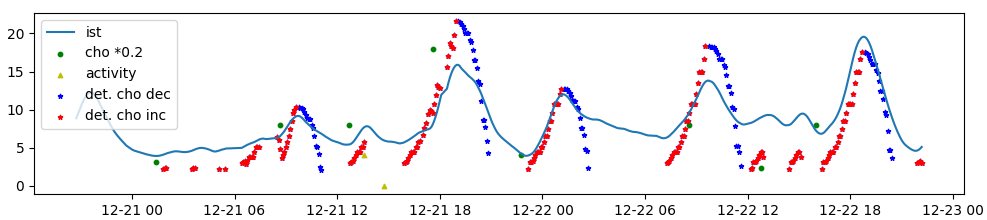
\includegraphics[width=1\textwidth]{img/cho/hrany.png}
\end{figure}

Jídlo je detekováno, pakliže aktivační funkce vzestupné hrany je větší než zvolený threshold. Nízký threshold detekuje většinu jídel, ale také může detekovat výkyvy nesouvisející s příjmem karbohydrátů. Naopak vysoce zvolený threshold nebude detekovat menší jídla. Řešením je použití více thresholdů pro stanovení pravděpodobnosti jídla.